\documentclass[12pt]{article}
\usepackage{epsfig,a4}
\usepackage{draftcopy}
\begin{document}
\thispagestyle{empty}
\title{CloudMan: design document Betelgeuze. Draft Version 0.92}
\author{CERN IT-DEP/PES-PS, BARC}
%\version{0.0.2}
\date{\today}
\maketitle 
\begin{abstract}
This document describes the design for the Betelgeuze release of CloudMan.

\end{abstract}
%
% contents
%
\tableofcontents
\listoffigures 
\listoftables

%
% introduction 
%
\section{Introduction}
CloudMan is a high level resource management tool which provides a central place to configure resources allocations in a computer center. Users who authenticate to CloudMan have privileges which depend on the role they have been assigned by somebody else. This way CloudMan allows for a delegation of configuration details to user communities. As an example, a CloudMan super user can create a new user group {\it A} and assign computing resources in specific parts of the computer center to this group of people. As an example, group {\it A} can correspond to the list of computing coordinators of a big LHC experiment. 
The people belonging to group {\it A} can decide themselves how they want to make use of those resources. Let's assume that the computer center offers two projects {\it X} and {\it Y} which are interesting for the user group {\it A}. Examples of those projects can be a classical batch system, providing resources which are available from the Grid, and a virtual machine self-service. So they decide to use 90\% of the resource for classical batch while the rest should be used for a self-service. 
As the people from group {\it A} are usually busy people, they can further delegate the  management of the resources within the project. They could found a batch group for the experiment which can give the bulk of the batch resources to the Higgs research group, and the rest to some students. 

The CloudMan front end takes care of the hierachies and privileges. The result of the allocation is exported in a machine readable format, and can then be used by scripts to configure the services behind the projects. 


%
% Purpose
%
Concepts and initial ideas of the CloudMan project are described in~\cite{CloudManProject}. The purpose of this document is to define interfaces and the design of the modules, aiming at the implementation of the tool. An overview over the architecture is given in fig.~\ref{architecture}, as described in ~\cite{CloudManProject}.

As a general guideline, standard OpenSource tools and frameworks, and/or existing services should be used where ever possible. 

\begin{figure}
\begin{center}
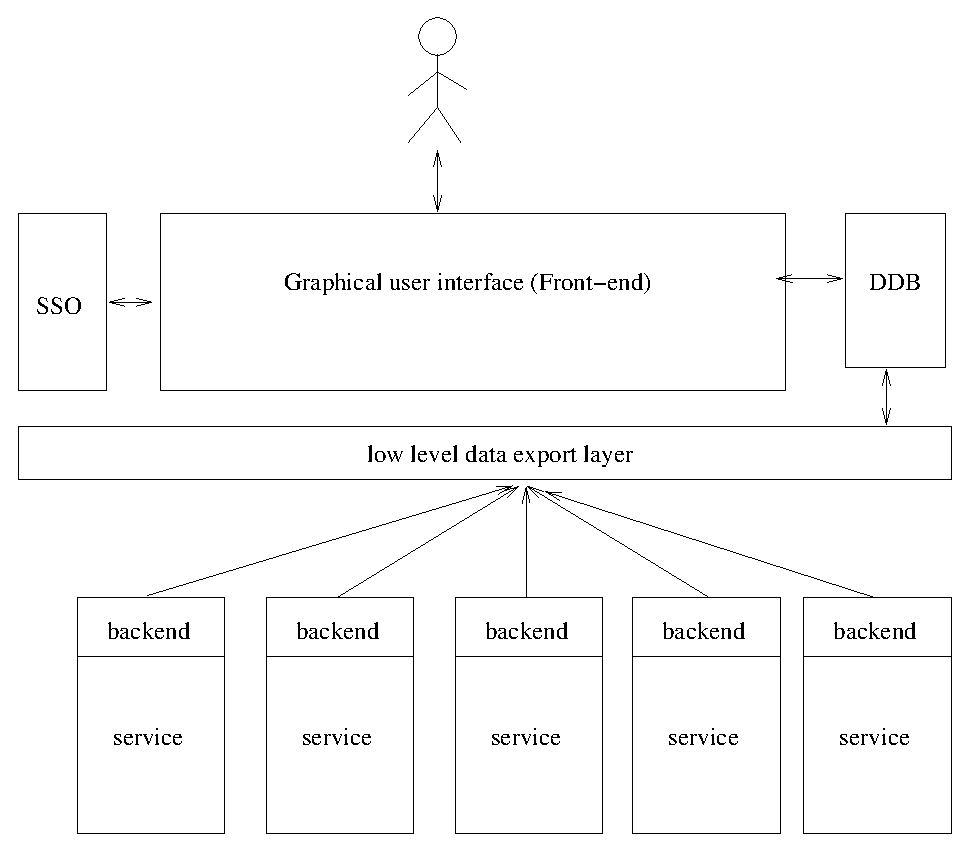
\includegraphics[width=0.9\textwidth]{architecture2.eps}
\caption{\label{architecture} Basic architecture of the desired system. Users connect to the front-end which offers a graphical user interface. They authenticate using the site Single Sign On mechanism or similar. The data which is entered is stored in an external database, and exported in a low level format. Back-ends which are design to configure specific services, for example local cloud installations, consume this information to configure their resources.}
\end{center}
\end{figure}



%
% terms and definitions
%
\section{Terms, definitions and concepts}
This section defines the terms which are used by CloudMan. 

\subsection{Regions}
A region in CloudMan can be single computer center or a set of computer centers making up a single entity, for example a site. Regions are distinct and independent computer centers. 

\subsection{Resource types}
In the Aldebaran release, a resource type was used as a minimal unit in which resources could be allocated. This idea turned out to be little useful, and added an unexpectedly large amount of additional issues. 

For Betelgeuze, resource types are redefined. We distinguish two different types:
\begin{itemize}
\item allocatable resources
\item not allocatable resources, or features
\end{itemize}
As an example, CPU resources are allocatable while the fact that machines in a specific zone (see below for the definition) have a UPS is a feature which cannot be allocated, that is you cannot sum them up and give a share of it to somebody as you can do for CPU or disk resources. 

Resource types are defined through the web interface and stored in the database. Not allocatable resources types require the following information:
\begin{itemize}
\item A name which identifies the resource. This name is used on the CloudMan interface when displaying the resource and it's usage. 
\item A floating point number indicating the price of this feature. The more expensive the resource is the higher the number should be. The aim of this number is to help the administrator to define the possible cost of resources in zones which provide this feature or resource. It must be possible to edit this number for existing resources. 
\end{itemize}
Allocatable resources require {\bf in addition} to the above the following information:
\begin{itemize}
\item A value (in general a floating point value)
\item A unit (stored as a string). This unit determines the unit in which the value is stored in the database
\item A list of alternate units along with a conversion rule which relates the new unit to the original one stored in the database 
\end{itemize}

As an example, {\it CPU resources} are measured in {\it HS06} which is a floating point number but can also be given in {\it kSi2k}. 
The actual value is filled in at the zone level, see below.

\subsection{Zones}
A zone is a specific part of a {\it region}. Each region is made up of one or more zones. As an example, a zone can map to a hardware installations with specific features, like batch nodes or machines for storage. 

A zone is defined by the allocatable and non allocatable resource which it provides. 
When a new zone is created, the administrator describes it by the different resources which it provides. For allocatable resources he needs to define the actual value of the resource (or amount of this resource) which is provided by this zone. 

A measure for the cost is defined for each zone as a floating point number. 
It is set manually when the zone is allocated, depending on its features and resources. The field must be editable, the unit is arbitrary. The higher the number, the higher the cost of resources in this zone.

{\bf Note:} Care must be taken in how zones in CloudMan are defined. Example: Let's assume that a site has two distinct computer centers. These computer centers are physically distinct, but the site runs a batch farm which spans over the two computer centers transparently to the users. In this case, all computing resources seen by the batch farm for public use should belong to the same zone in the CloudMan sense. Else, top level allocations could set additional quotas which may result in a fragmentation of resources. 

The relationship of regions and zones for a case like  CERN with several computer centers is shown in fig.~\ref{cerncase}.
\begin{figure}
\begin{center}
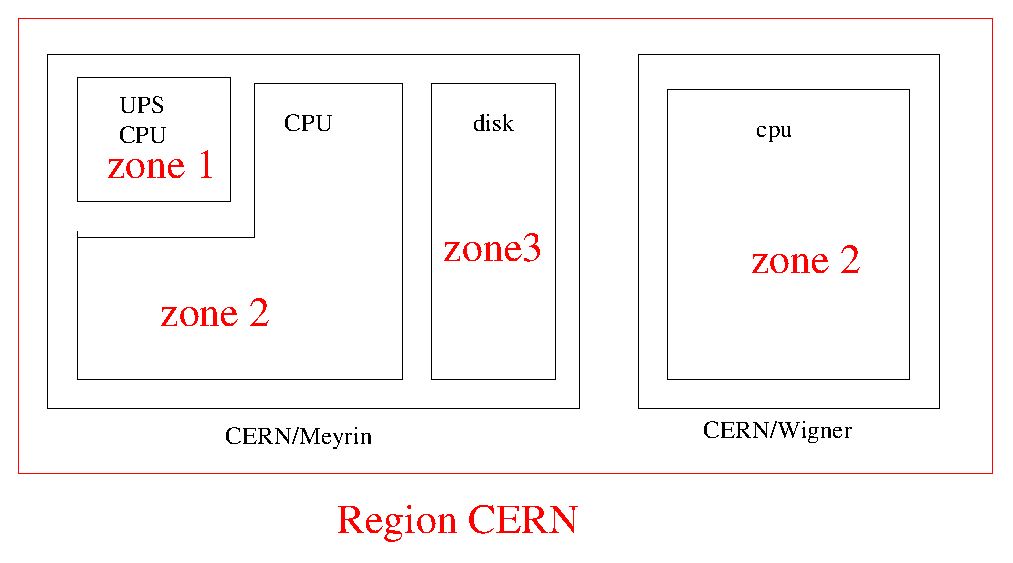
\includegraphics[width=\textwidth]{cerncase.eps}
\caption{\label{cerncase}Simplified scenario for CERN. It is assumed that there are two distinct computer centers which look like one large site. As an example the batch resources spread over the two computer centers. Therefore, only one region is present. Within this region there are CPU resources under UPS coverage, cheap CPU resources and disk resources. Similar resources which spread over the different computer centers still belong to the same zone.}
\end{center}
\end{figure}

\subsection{Groups}
In the previous release of CloudMan there was the concept of groups. For the CERN deployment, groups are handled by e-groups, therefore the CloudMan groups were nothing but a pointer to e-groups. As of Betelgeuze this concept is dropped and replaced by directly giving the e-groups name.

\subsection{Top level allocations}
In the CloudMan configuration files, it is possible to define a group of CloudMan administrators. These people are the only once who are allowed to perform top level allocations. A top level allocation is the assignement of a specific quantity of a resource to a user group. Top level allocations are done per zone and region. This way top level allocations set quotas on the possible usage of specific zones. 
\begin{table}[htb]
\begin{center}
\begin{tabular}{|l|l|l|l|}
\hline
Zone & total & experiment name & allocation \\
\hline
Nr. 1, UPS covered & 10 servers, 100HS06 each & CMS &  100 HS06 \\
Nr. 2, simple CPU  & 100 servers, 100HS06 each & CMS & 900 HS06 \\
\hline
\end{tabular}
\end{center}
\caption{\label{toplevelCMS}Example top level allocation for CMS: There are two zones, one with UPS coverage which has 10 servers, and one with 100 servers for CPU processing. The performance of each server corresponds to 100~HS06. CMS gets a total allocation of 1000~HS06, 10\% of which are UPS covered.  Cost of resources in zone 1 are larger than those in zone 2 due to the UPS feature.}
\end{table}
An example top level allocation is shown in table~\ref{toplevelCMS}.

\subsection{Projects}
A project is a service which is provided by the computer center and to which users can subscribe, in case they have got a top level allocation which is required for this service. Only CloudMan admins can create projects.  As an example, a computer center can offer computing resources in a batch farm so the CloudMan administrator would allocate a project {\it batch} to which all user groups who got a top level computing resource allocation can sign up. 

Table~\ref{projects} gives an example of project 
\begin{table}[htb]
\begin{center}
\begin{tabular}{|l|l|l|l|}
\hline
Project name & requirements & attributes & limitations\\
\hline
public batch & CPU resources & SHARE & maximum recursion depth 2 \\
vobox & CPU resources, UPS coverage & none & none \\
IaaS self service & CPU resources & none & none \\
\hline
\end{tabular}
\end{center}
\caption{\label{projects}Example projects which are allocated by the CloudMan administrator. There are 3 only here: public batch is owned by some group in IT which manages the batch farm. The idea of this project is to setup shares for large user groups. The vobox project is a service where experiments can get reliable resources which are covered with a UPS. This project will only use resource from Zone 1 in fig~\ref{cerncase} while the batch project will use only resources from Zone 2 because they are cheaper. The attribute SHARE indicates that these are shared (not dedicated) resources. The maximum recursion depth means that for this project it is possible to do group and subgroup allocations only, and not beyond that. The IaaS self service is meant for cheap development machines. It uses the same resources as the public batch project.}
\end{table}

\subsubsection{Project requirements}
In general, different projects will come with different service level agreements (SLA). In order to be able to fulfill these SLAs some projects will require specific features for the resources to be allocated to them, and thus enable only specific zones. 
When selecting resources , the cheapest matching option should be chosen to allocate resources. 
As an example, a site may run a batch farm and a service for critical applications. There will be two projects: a batch project with a requirement to select CPU resources, and a VOBOX\footnote{This is a CERN specific term for a service to give resources for critical applications to user communities/experiments} service which will require UPS coverage. 

\subsubsection{Project attributes}
When creating a project it must be possible to define attributes. An attribute is a key-value pair which is required to configure the project. At the project level it must be possible to provide a default value which is used if the user does not provide a value when assigning resources to this project. 

Project attributes are exported as key-value pairs so that they are available to the backend which configures the project. 

\subsubsection{Recursion limitation}
A special project attribute is a limitation on the recursion deps. By default there is no limitation on the maximum depth on group and subgroup allocations. In order to keep the complexity of some of the backends limited it may be necessary to restrict such allocations down to the subgroup level, for example. 


\begin{table}[htb]
\begin{center}
\begin{tabular}{|l|l|l|}
\hline
Project name & Administrator & Allocation \\
\hline
public batch & CMS\_batchadmin& 80\%\\
vobox & CMS\_VOC & 10\%\\
IaaS self service & CMS\_all& 10\% \\ 
\hline
\end{tabular}
\end{center}
\caption{\label{projectsAllocation} Project allocation for the example CMS group. These allocations are done by the CMS administrator who can sign up to any project for which he has a matching resource allocation. For each project he's interested in he determines a responsible (group of people), and gives them a fraction of the resources he got from the CloudMan administrator. With 10\% of the total allocation in the UPS they fill up their quota there.}
\end{table}

\subsection{Project allocations}
A project allocation is an assignement of resource to a specific project. This can be done by any member of a group which got a top level allocation for a resource which is required by the project. A project allocation is taken from a top level allocation for a specific project. When doing a project allocation a group of people the project allocation managers  have to be specified who will manage this project allocation in the future.

Table~\ref{projectsAllocation} gives an example of how a project allocation works. 

\subsection{Group and sub-group allocations}
Project allocation managers got an allocation of resources for a specific project. These people can delegate further management of these resources to another group of people who in turn can reallocate their bit of the cake to other people (sub-group allocations). 
The maximum depth of group, subgroup, sub-subgroup etc allocations is a feature which is project specific. It must be possible to restrict the recursion depth per project. This is illustrated in table~\ref{groupAllocationForBatch} and ~\ref{subgroupAllocationForBatch} for the batch project in our example.

\begin{table}[htb]
\begin{center}
\begin{tabular}{|l|l|l|}
\hline
Group name & Administrator & Allocation \\
\hline
HiggsSearchers & CMSHiggsAdmins& 80\%\\
Other & CMS\_batchadmin & 20\%\\
\hline
\end{tabular}
\end{center}
\caption{\label{groupAllocationForBatch}Group allocations for the batch project as done by the CMS\_batchadmin. The Higgs search group gets a large share of the batch system share of CMS. They can further on set priorities by defining shares for the individual Higgs search teams.  }

\end{table}

\begin{table}
\begin{center}
\begin{tabular}{|l|l|l|}
\hline
SubGroup name & Administrator & Allocation \\
\hline
HiggsChannelA & CMSHiggsAdmins& 25\%\\
HiggsChannelB & CMSHiggsAdmins& 25\%\\
HiggsChannelC & CMSHiggsAdmins& 25\%\\
HiggsChannelD & CMSHiggsAdmins& 25\%\\
\hline
\end{tabular}
\end{center}
\caption{\label{subgroupAllocationForBatch}Group allocations for the batch project as done by the CMS\_batchadmin. The Higgs search group gets a large share of the batch system share of CMS. They can further on set priorities by defining shares for the individual Higgs search teams. Due to the limitation in the recursion depth in the batch project it is not possible for the CMSHiggsAdmins to further split up the resources. }
\end{table}

\subsubsection{Group and subgroup attributes}
Group and subgroup allocations belong to a specific project. When doing such an allocation, it must be possible to update the values of the attributes which are required by the project. If no new value is given, it is inherited from the hierarchy above.  


\section{Buisiness continuity}
If a site has two distinct computer centers it may want to distribute all services in a way which allows it to continue to work even if one of the two centers goes down. Services and applications have to be able to support such a scenario. From the infrastructure point of view it requires that all relevant services to have one leg in each of the computer centers. 
In a fully virtualized computer center this requirement is one on the scheduling policies: instead of filling up hypervisors one by one VMs belonging to the same project have to be distributed over the two centers. 

In Cloudman this can be done if all zones for the relevant services spread over the two computer centers. Projects supporting this option should have a flag which indicates that the resources should be distributed over the two centers rather than being filled up one by one. The flag is implemented as a special project attribute. This will be visible from the low level export layer to the backend which configures the project. 





%
% goals of phase 1
%
\section{Implementation goals}
The aim of this design phase of the project is the implementation of 
\begin{itemize}
\item The graphical user interface 
\begin{itemize}
  \item the GUI itself is stateless
  \item all data is kept in a database backend (mysql,oracle)
  \item the GUI is accessible behind a (load balanced or round robin) alias. For example, at CERN one instance can be run at Meyrin, the second at SafeHost, thus providing redundancy.
  \item the application is implemented in Django\cite{Django} framework, running on an Apache web server with Shibboleth for implemeting SingleSignOn   
  \item access is secured via SSL. For the CERN instance, CERN provides a certificate signed by the CERN CA.
  \item Low-level data export is visible inside CERN without authentication.
  \item projects are associated to a project backend which consumes the data and provides state data. When allocating the project it is mandatory to provide the location for the state data. The state data format is fixed
  \item a cron job on the CloudMan server regularly reads the state data for all projects and records it in the database
  \item the GUI provides a way to present current state data per project
  \item the GUI provides a way to present historical state data per project, including configuration errors or problems 
\end{itemize}
\item The database backend
\begin{itemize}
  \item Oracle or Mysql are preferred
  \item the database access is abstracted using the Django Object Relational Model (ORM)\cite{ORM}; writing direct SQL statements is to be avoided
  \item the backend database should have transaction support to insure data integrity when doing multiple updates. Django Object Relational Model (ORM)\cite{ORM} transaction support can be used.
\end{itemize}
\item Authentication
\begin{itemize}
\item It must be possible to use CERN SSO~\cite{CernSSO} to authenticate users. The CERN instance will only use this mechanism for authentication
\item Access will stay in SSL secured after login
\end{itemize}
\item Authorization
\begin{itemize}
\item cloudMan does not use Unix group IDs, and relies only on e-groups or user name lists
\item there is one and only one resource manager role
\item the name of the resource manager group is defined in the CloudMan configuration file and is therefore a configuration option 
\item ordinary users only have access to information within their hierarchy. 
\item the role of a user is determined by the e-groups~\cite{CernEgroups} he belongs to
\item the use of e-groups~\cite{CernEgroups} allows to move much of the complexity due to the hierarchy of roles into this existing service
\item the e-groups used for mapping users to roles must be configurable via the GUI, respecting ACLs and hierarchies
\item in case e-groups is not available (eg outside CERN), simple lists of users can be supported
\end{itemize}
\item data export level
\begin{itemize}
\item the backends will pull the information required to configure themselves from the low level data export layer which is fed by the GUI. 
\item the backend will report back on the  current resource consumption as well as possible configuration problems. The data is provided on a shared file system or a URL. The location of the state data is defined for each project
\item the location of the state data for each project can be changed by the CloudMan administrators. 
\item if the exported data contains fields which are not supported by a backend, the backend can ignore this data
\item the data export is done in a machine readable way, eg via a XML,JSON,yaml format. 
\item the data export is SSL secured 
\item all changes done in the front end must be traceable, including information about 
\begin{itemize}
 \item what has been changed 
 \item what operation has been done 
 \item when it has been changed
 \item who applied the change
\end{itemize}
\end{itemize}
\item if time allows sample backends for the following possible projects should be provided
\begin{itemize}
\item a sample backend to configure OpenStack
\item a sample backend to configure OpenNebula
\item a sample backend to configure batch resources 
\item a sample backend to configure storage (AFS, EOS or CASTOR) 
\end{itemize}
\end{itemize}
All backends must support a no-action mode, as well as different logging levels (info, error, debug), ideally through syslog.



%
% Use cases
%
%\section{Use cases}
%CloudMan will be used to manage an IaaS based computer center layout, as shown in figure~\ref{iaas}. The use cases naturally derive from this model. In this picture, each application comes with a backend which uses information from CloudMan to configure itself, respecting the allocations of resources to each defined user community.
\begin{figure}
\begin{center}
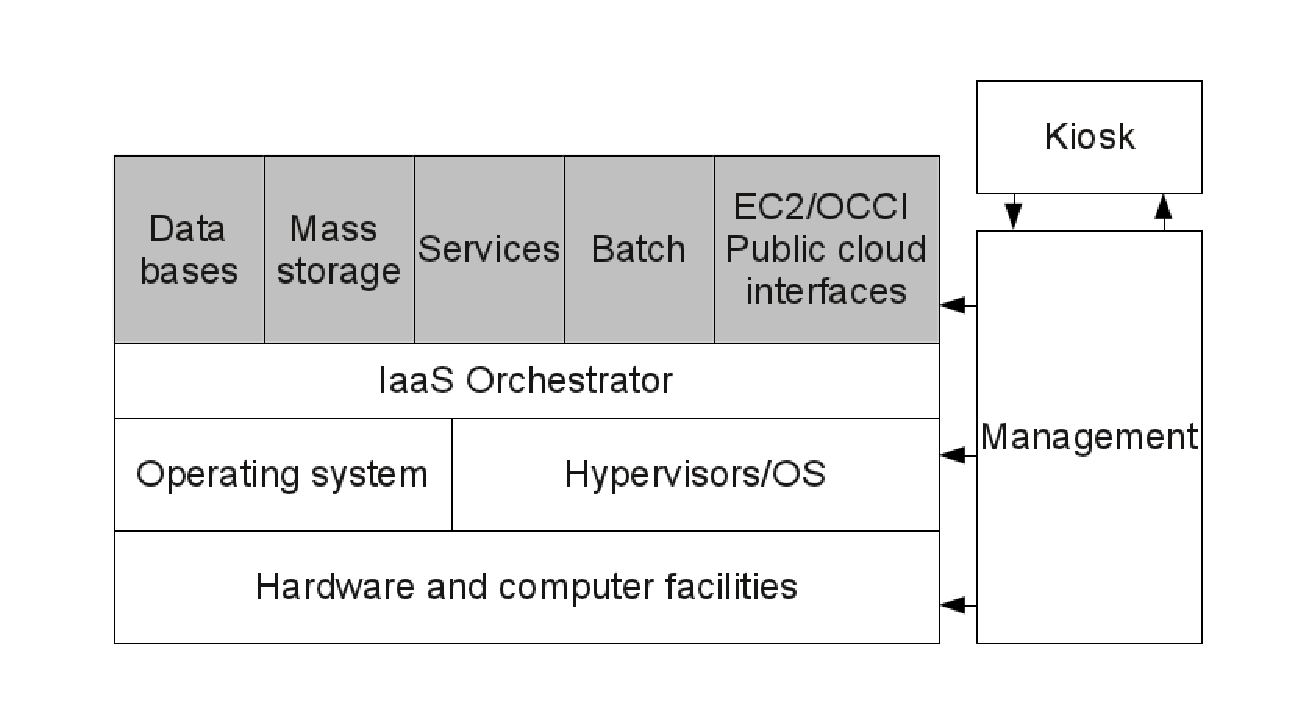
\includegraphics[width=\textwidth]{iaas.eps}
\caption{\label{iaas}Vision of a high level structure for an IaaS based computer center. CloudMan will be an essential part of the management layer for this model.}
\end{center}
\end{figure}
CloudMan must be capable to cope with the configuration of the use cases:
\begin{itemize}
\item Global allocations for individual IT services like 
\begin{itemize}
\item lxbatch resources, physical and virtual~\footnote{These correspond to different resource pools} 
\item public cloud resources for general use
\item storage resource pools for CASTOR and SWIFT
\item storage resource pools for virtual batch scratch and AFS cache space
\item physical resource pools for databases
\end{itemize}
\item The configuration of quotas per VO for an EC2 based self-service
\item The enforcement of quotas for reliable resources, based on total resources per VO by the resource manager
\item The configuration of shares for the batch farm VO project admins and subproject admins
\begin{itemize}
 \item The total resource allocation, typically in kSi2K for shared batch resources is done directly by the resource manager 
 \item The resource manager only defines a global allocation for each VO for resource pools used by the batch farm
 \item The difference between allocations done for the VOs and totally available resources for lxbatch are used for a public share
 \item The VO responsibles for projects and subprojects decide for which applications these resources are used. The fraction of resources allocated to batch processing is translated by the corresponding backend into a fair share value.
\end{itemize}
\end{itemize}

The following specific use cases are identified:
\begin{itemize}
\item new CPU resource have arrived for use by the self service
\item the fraction of SLC5 and SLC6 resources in lxbatch needs to be changed 

\end{itemize}



\section{Backend types}
Backends are plugins to CloudMan which can and should be shipped separately from the CloudMan interface itself. Backends are in general expected to be site specific. The base distribution of CloudMan should provide a framework for developing backends. Optionally, it  can ship sample implementations to document how to use the framework.

We distinguish two different classes of backends:

\begin{itemize}
\item {\it Project backends} are project specific scripts which consume only the data specific to the project they belong to. 
\item A {\it Mover} is responsible for resource sharing between different backends. 
\end{itemize}

\subsection{Project backends}
For each project there will be one and only one project backend. The project backend consumes data related to the project for which it has been designed. The CloudMan frontend must be able to query the current status of the configuration. This will allow the administrators to watch the status of any change requests done, and verify the integrity of the data which has been entered. 

State data is published in a simplistic way, either a file on a shared file system, or a URL. 

Adding support for project backends results in the following requirements:
\begin{itemize}
 \item when allocating a new project the backend has to be specified along with the source of the state data 
 \item a cron job on the CloudMan front end regulary reads  the state data for all project backends and put it into a database table to record historical information
 \item when a user queries state data from the GUI the information is taken from the state data source, not from the database
 \item the CloudMan front end needs to offer a way to display the current state data per project
 \item the CloudMan front end needs to offer a way to display the historical evolution of the state per project 
 \item all project backends must publish their state data in a common and agreed format
 \item project backends need to provide an interface which allows automatic shrinking of resources
\end{itemize}

\subsection{Mover backend}
In a full CloudMan installation there should be one mover backend. It is responsible to shift resources between different projects. Therefore, it has to match the following requirements:

\begin{itemize}
 \item the mover backend needs to have access to the state data of each project between which it is supposed to shift resources
 \item the mover backend reads the list of projects along with the project state data from the CloudMan export layer
% \item where to define the mover backend in CloudMan
% \item try to have only one mover
% \item name and source of state info defined in configuration file of CloudMan ?
% \item for some projects a plugin will be needed to manage resources, eg draining of nodes, or claiming back VMs
\end{itemize}
The mover can be implemented as a scheduler on the CloudMan front end which triggeres actions on Project backends. 

%Possible backends include 
%\begin{itemize}
%\item One or more plugins to configure batch system shares, one per batch system in use (eg LSF, SLURM, ...)
%\item One or more plugins to configure an OpenNebula instance
%\item One or more plugins to configure an OpenStack instance
%\end{itemize}
%Plugins are expected to be project driven but they don't have to be. This is specifically true for plugins which talk to
%an internal cloud setup: A site may choose to have one plugin for each tenant in an OpenStack instance, or rather use
%only one plugin which will configure the whole cloud instance. 


%\section{Benefits, assumptions, risks/issues}
%Writing backends for Cloud controllers like OpenStack and Opennebula bears some risk as the concepts and definitions used by those young projects are still changing rapidly. In addition, the backends for these systems will be very model dependent, in the sense that each site who deploys them will configure them differently. 

 


\section{Project backend examples}
Sample implementations of project backends are listed in the following sections.
\subsection{Batch shares}
CloudMan should support the definition of shares for a batch processing project. 
Such a backend is particularly interesting for CERN because there is already an
existing application ({\it LSFweb}) which has been designed before SSO and 
egroups were introduced at CERN. The new backend will allow to replace this old 
tool. 

When determining resources for a batch farm, there are two aspects which need
to be considered:

\begin{enumerate}
\item the batch processing resources: The batch farm itself has a certain size, that is a number of worker nodes providing job slots, which are available for the users to process their data. In the simplest case all worker nodes are organized in a single public partition which can be accessed by all registered users. At CERN, the situation is more complicated though. Although all CPU resources belong to the same batch instances, there are additional partitions providing dedicated resources to some user groups. 
The bulk of computing resources at CERN consist of physical worker nodes. The configuration of these resources is currently done using the Quattor tool kit. At the long term there are plans to virtualize more and more of these resources, and provide them through an internal cloud. It should be possible to use CloudMan to manage such resources, for example through a batch resource project. 
 
\item the user shares: Some of the batch partitions implement fair share. At CERN, batch shares are currently managed through a graphical user interface called
LSFweb. It should be possible to manage LSF shares through a batch project from CloudMan, allowing to replace the old LSFweb tool.
\end{enumerate}

CloudMan shall offer a way to configure both batch resources and batch user shares from a single interface. 

The goal for the first design phase is to develop a prototype of a backend for the second use cases. Ideally, some tools should be provided which allow to migrate from LSFweb to CloudMan in an easy way.

\subsection{Cloud drivers: common ideas}
In this section ideas to configure a small cloud infrastructure are discussed. More complex environments will require a more detailed discussion. What is proposed here is meant to be a proof of concept. 

When designing cloud driver backends for CloudMan, two different aspects of resource management need to be respected. 

\begin{enumerate}
\item Setting quotas and ACLs for a the cloud infrastructure within projects or tenants
\item Moving resources between different projects
\end{enumerate}

The first case only deals with quotas and user groups inside an IaaS cloud.

The second case can only work if all projects share the same resources. The example use case is a small infrastructure which provides resources for a public cloud interface and a virtual batch farm which run on the same resources. 


\subsubsection{A possible model}
For the prototype driver we only consider 2 cases: a public batch farm and a EC2 based self-service.

The model to be implemented looks like this:
\begin{enumerate}
\item The Cloudman adminstrator defines a top level allocation per user group, and defines the administrator e-group for this allocation. This allocation is the total resource allocation (in HS06) for the user community. For CERN, user communities are ATLAS, CMS, SFT, IT, ...
\item The CloudMan administrator defines a new project (eg IaaS Self-Service). 
\item Initially, all resources are allocated to batch
\end{enumerate}

\subsubsection{Self-service configuration}
Group administrators can sign up to the IaaS Self-service by doing a project allocation from their top level allocation. In order to do so, they  need to reduce the batch capacity. The group administrator can then create group and subgroup allocations for the EC2 access resulting in a tree like structure as he needs it.
Egroups are to be resolved on the CloudMan Frontend.
The backend can then consume the leaves of this tree, which contain lists of users. It will use these user lists to create groups of users. The resource allocations for these user groups are used to setup group quotas. 

\subsubsection{Conversion of units}
In CloudMan CPU resource allocations are done in HS06 (or equivalent) while quotas on cloud infrastructures are typically done in number of machines, virtual CPUs or 
the like. Zones will usually consist of hypervisors with different HS06 ratings. The conversion of HS06 quotas into a quota on the number of virtual machines adds a bit of complexity to the backend. Further discussion on this is required. 


\subsection{OpenStack}
The planned OpenStack backend can be derived from the OpenNebula backend. Projects will be mapped to tendants. 
As in the OpenNebula case, the backend will create a new tenant for each leaf in the tree defined in CloudMan.

Thus, the OpenStack backend relies on the possibility to set quotas per tenant. 
 

\subsection{OpenNebula}
%The OpenNebula backend is meant mainly as a playground until an OpenStack testbed is available. 
With the availability of an OpenStack testbed the priority of developing a backend for OpenNebula has dropped for CERN. The OpenNebula based infrastructure at CERN is planned to be retired at end 2012 or early 2013, and absorbed in the new OpenStack based infrastructure. Therefore the priority is moved to OpenStack. 





\section{Storage}
At CERN, different storage solutions are in place. Resource allocation for the existing storage solutions is often done already in a hierarchical way, similar to the ideas of the CloudMan design. 

The storage solutions at CERN have special requirements though. These are summarized in this section.

\subsection{AFS}
At the time of writing this document, AFS resources at CERN are managed like this:

\begin{itemize}
\item the AFS service provide so called "project spaces"
\item in 1st approximation project spaces are defined by a project name, e.g. "atlas", a path, e.g. "/afs/cern.ch/atlas", and a quota, "e.g. 10TB"
\item the management of the project spaces is outsourced to so-called project admins
\item being a project admin basically means being member of the AFS group "\_projectname\_", e.g. "\_atlas\_"
\item project admin's task include
\begin{itemize}
    \item creating/deleting different types of volumes
    \item managing ACLs
    \item managing readonly volumes
\end{itemize}
\item tool to manage all this is afs\_admin (running it as an admin of a project w/o any option will list all the subcommands)    
\end{itemize}

The AFS service managers see a possible benefit in managing at least parts of the AFS resource~\cite{arne}. In particular:

\begin{itemize}
\item quicker overview of the managed AFS project space
\item easier to execute specific commands (e.g. if CloudMan "knows" to required parameters and can do some sanity checking)
\end{itemize}

Requirements for a potential web-interface include:

\begin{itemize}
\item CloudMan cannot be the primary source of any information, so it must be able to retrieve information from somewhere else (like parsing a file or running a command)
\item CloudMan must be able to somehow trigger a authenticated command (afs\_admin) on behalf of the user
\item CloudMan must be able to give feedback to the user if a command succeeded or not
\item extending/changing afs\_admin should not require changes in CloudMan and it should support the full command set
\item AFS project administration is based on AFS groups, not e-groups, so CloudMan needs to either grab that info from the AFS group or establish a sync from AFS into e-groups 
\end{itemize}

\subsection{EOS}
On EOS each experiment has dedicated resources. Unlike castor, eos has quota and it manage the quota
in a kind of tree structure. In the eos case we have the same admins as in castor and they can assign quota to
a particular tree and to a particular user/group or e-groups, decide the file replication level and other attributes.
All the space/file quota and the access/ACLs are done by these few admin which use the eos shell.

For the procedure to shift resources from CASTOR to EOS (or viceversa) is done by hand just draining and reinstalling the diskserver in the correct cluster.
In general we base our diskserver allocation on the 2012 pledge of the experiment and then we decide in a meeting with them were to allocate the new resources (which castor svclass or EOS) according with their needs.


Potential benefit we can gain from CloudMan is a graphic interface to eos (we probably need to check with the few admin if they do this by hand or via some script), for castor could only be useful for setting up the permission on the svclass. On the other hand I think CloudMan would be very helpful for having a general view on the experiment resources (where the space is allocated) but this raw information (like AFS) should be retrieved direcly from castor or eos.

\subsection{CASTOR}
We have 5 different CASTOR instances (atlas, cms, alice, lhbc, public)
each of them has its own resource (diskservers). The resources are divided into service class (svcclass which are mapped as separate subclusters/pools).
For example in c2atlas (the atlas instance) there are 7 svcclass:
t0atlas, t0merge, atlcal, etc..
In general we discourage to create new svcclass (Except for new "big" experiment in castor public e.g. ams)

User have the privilege to store data only via their experiment resources, we have kind of "acl" at the svcclass level.
We delegate the power of setting these rules to specific person that are the group admin. In this case the admin can decide which commands users can run (stager\_get, recall, ..) 
Unfortunately in castor there is no easy way to manage quota, we only manage the resources (diskservers installed) in a particular svcclass (diskpace)

%\subsubsection{Configuration files}
%Static configuration data can be stored in configuration files on the 
server(s) but should be avoided, in order to keep the service stateless. 
Instead, such configuration data should be entered in the GUI and 
stored in the database. 

In case such a file is needed anyway, the format must be plain text, 
so that it can be easily manipulated by configuration components
 eg from Quattor (or Puppet). The development of such 
components is NOT part of this project. The format must be key-value pairs, 
following the python config parser format {\it FIXME: add reference}
 
 




%\section{Resource pools}
%Resource pools in CloudMan only have high level meta data information, like
\begin{itemize}
\item identifier (eg like landb cluster name)
\item description
\item size 
\item type
\item features 
 \begin{itemize}
 \item public or not
 \item support for life migration or not
 \item reliable or not, critical power etc 
 \item GPN/LCG network
 \item {\it what else }
 \end{itemize}
\end{itemize}
There are mandatory and optional fields. 
It must be easy to add additional fields without having to 
change the application.
 



%
% details
%
\section{Details}
This section describes the details necessary for the implementation of the different modules.

\begin{figure}
\begin{center}
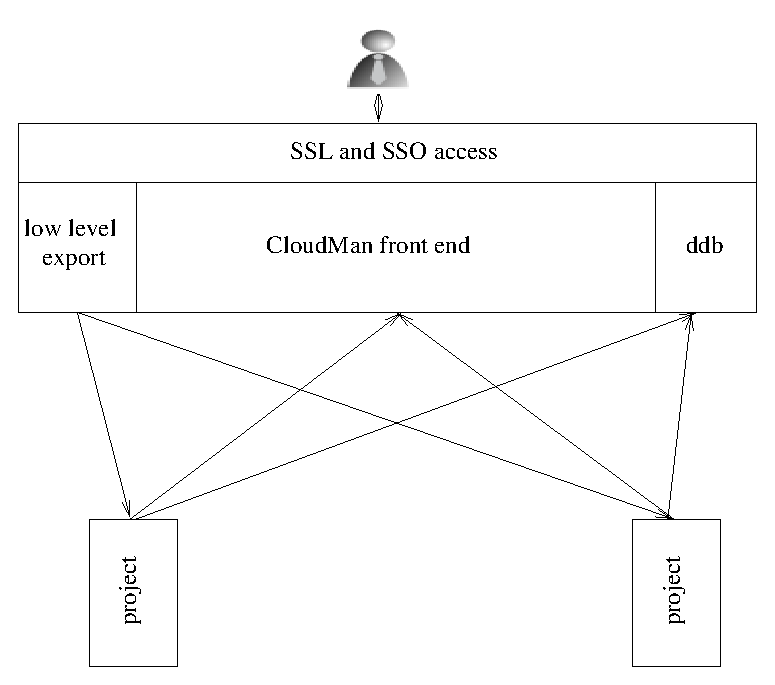
\includegraphics[width=0.9\textwidth]{cloudman_highlevel.eps}
\caption{\label{architecture} Updated architecture of the desired system. Users connect to the front-end which offers a graphical user interface. The side is secured with SSL techniques. All users have to authenticate using the sites Single Sign On mechanism. The data which is entered is stored in an external database and exported in a low level format. Shown in this figure are project specific backends only. In general these backends are site specific, and design to configure specific services. Each backend reads the data which it needs to configure it's resources from the low level export layer from CloudMan. The current state which includes error or warning conditions is reported back to the frontend as well as the CloudMan database. The database is used to record the historical state data per project backend.}
\end{center}
\end{figure}
Fig.~\ref{architecture} shows an overview over the CloudMan architecture. Users have to authenticate using SSO. After login, the communication stays secured by SSL. Project backends report their state asynchronously via a file or URL. The state data is recorded in the database to save the history. 


\subsection{Definition of Interfaces}

\subsubsection{Low level data export layer}
The low level data export layer publishes the configuration data entered in the front end, so that it can be consumed by the different backends.
The data and the format should be customizable for each backend. 
This can be done for example by exploiting features of Django.  

In the second phase of the project, the same mechanism shall be used by the backends to provide live monitoring information about their current status.




\subsubsection{Backend state data}

\begin{table}[bh]
\begin{center}
\begin{tabular}{|l|l|l|}
\hline
key& value type & values \\
\hline
\hline
ProjectName  & string &  Name of the project which this backend configures\\
BackendState & string &  one of [OK, WARNING,ERROR] \\
SampleTime   & seconds & Unix time stamp of when this sample was taken \\
BackendStateInfo& string & Free text \\
\hline
\end{tabular}
\end{center}
\caption{\label{stateinfo}Current state information as published by the project backends.}
\end{table}

\begin{table}[bh]
\begin{center}
\begin{tabular}{|l|l|l|}
\hline
key & value type & values \\
\hline
\hline
ResourceName& string & name of the resource \\
ResourceOwner& string & list of users or e-group\\
             &        &   to which the resource is allocated \\
ResourceAllocatedUnit & string & the unit \\
& & in which the resource is measured \\
ResourceAllocatedTarget & floating point & the target value for the \\
& & resource as demanded by CloudMan \\
ResourceAllocatedCurrent & floating point & the current value for the \\
& & resource as demanded by CloudMan \\
\hline
\end{tabular}
\end{center}
\caption{\label{resourceinfo} Required key-value pairs for state information as published by the project backends for each resource. The block is repeated for each ResourceOwner.}
\end{table}

\begin{table}[bh]
\begin{center}
\begin{verbatim} 
{
"ProjectName": "batch"
"TimeStamp": 1348218423
"BackendState": "OK"
"BackendStateInfo": "All OK"
"Resources":[
    {
       "ResourceName":"CPU",
       "ResourceOwner":"user1,user2,user10",
       "ResourceAllocatedUnit":"HS06",
       "ResourceAllocatedTarget":"1000",
       "ResourceAllocatedCurrent":"1000"
    },
    {
       "ResourceName":"CPU",
       "ResourceOwner":"user5,user6,user999",
       "ResourceAllocatedUnit":"HS06",
       "ResourceAllocatedTarget":"10",
       "ResourceAllocatedCurrent":"10"
    },
    {
       "ResourceName":"disk",
       "ResourceOwner":"user5,user6,user999",
       "ResourceAllocatedUnit":"GB",
       "ResourceAllocatedTarget":"500",
       "ResourceAllocatedCurrent":"500"
    }
 ]
}

\end{verbatim}
\end{center}
\caption{\label{messageformat} Example of backend state data  in JSON format }
\end{table}


Each project backend can publish state data as a flat file which can be located on a shared file system, or which is exported by a web server. The location of the state data as well as its format has to be specified for each project when defining the backend in the form of an URL~\footnote{eg. '' file://afs/cern.ch/project/.../input.json''}. Supported formats include YAML, JSON and XML.

The state information must include the key-value pairs listed in table~\ref{stateinfo}. Optionally, additional fields can be published. These can be displayed by the front end as additional information but have no influence on any actions taken on the frontend. The information in table~\ref{stateinfo} is published once per project backend. 

In addition for reach resource which is allocated to a project the information as described in table~\ref{resourceinfo} has to be published. The block in this table is repeated for each {\it ResourceOwner}. 
An example output in JSON format is given in table~\ref{messageformat}.


\subsubsection{CloudMan database schema}
An SQL database is used for the backend database. 

The following information is required:
\begin{itemize}
\item Super User name or e-group
\item Resource definitions and units
\item Resource features 
\item Roles
\item Map of user names or e-groups to roles
\item Table with historical state data for all project backends
\end{itemize}

The database holds all dynamic information. Static configuration data goes into the configuration files, see there. 
Certain information like the meta data of resource pools may change during the lifetime of the product. The database schema is made in such a way that it is easy to add or remove features which were not there at the beginning to the schema without having to perform complicated and slow database operations. 

\begin{figure}
\begin{center}
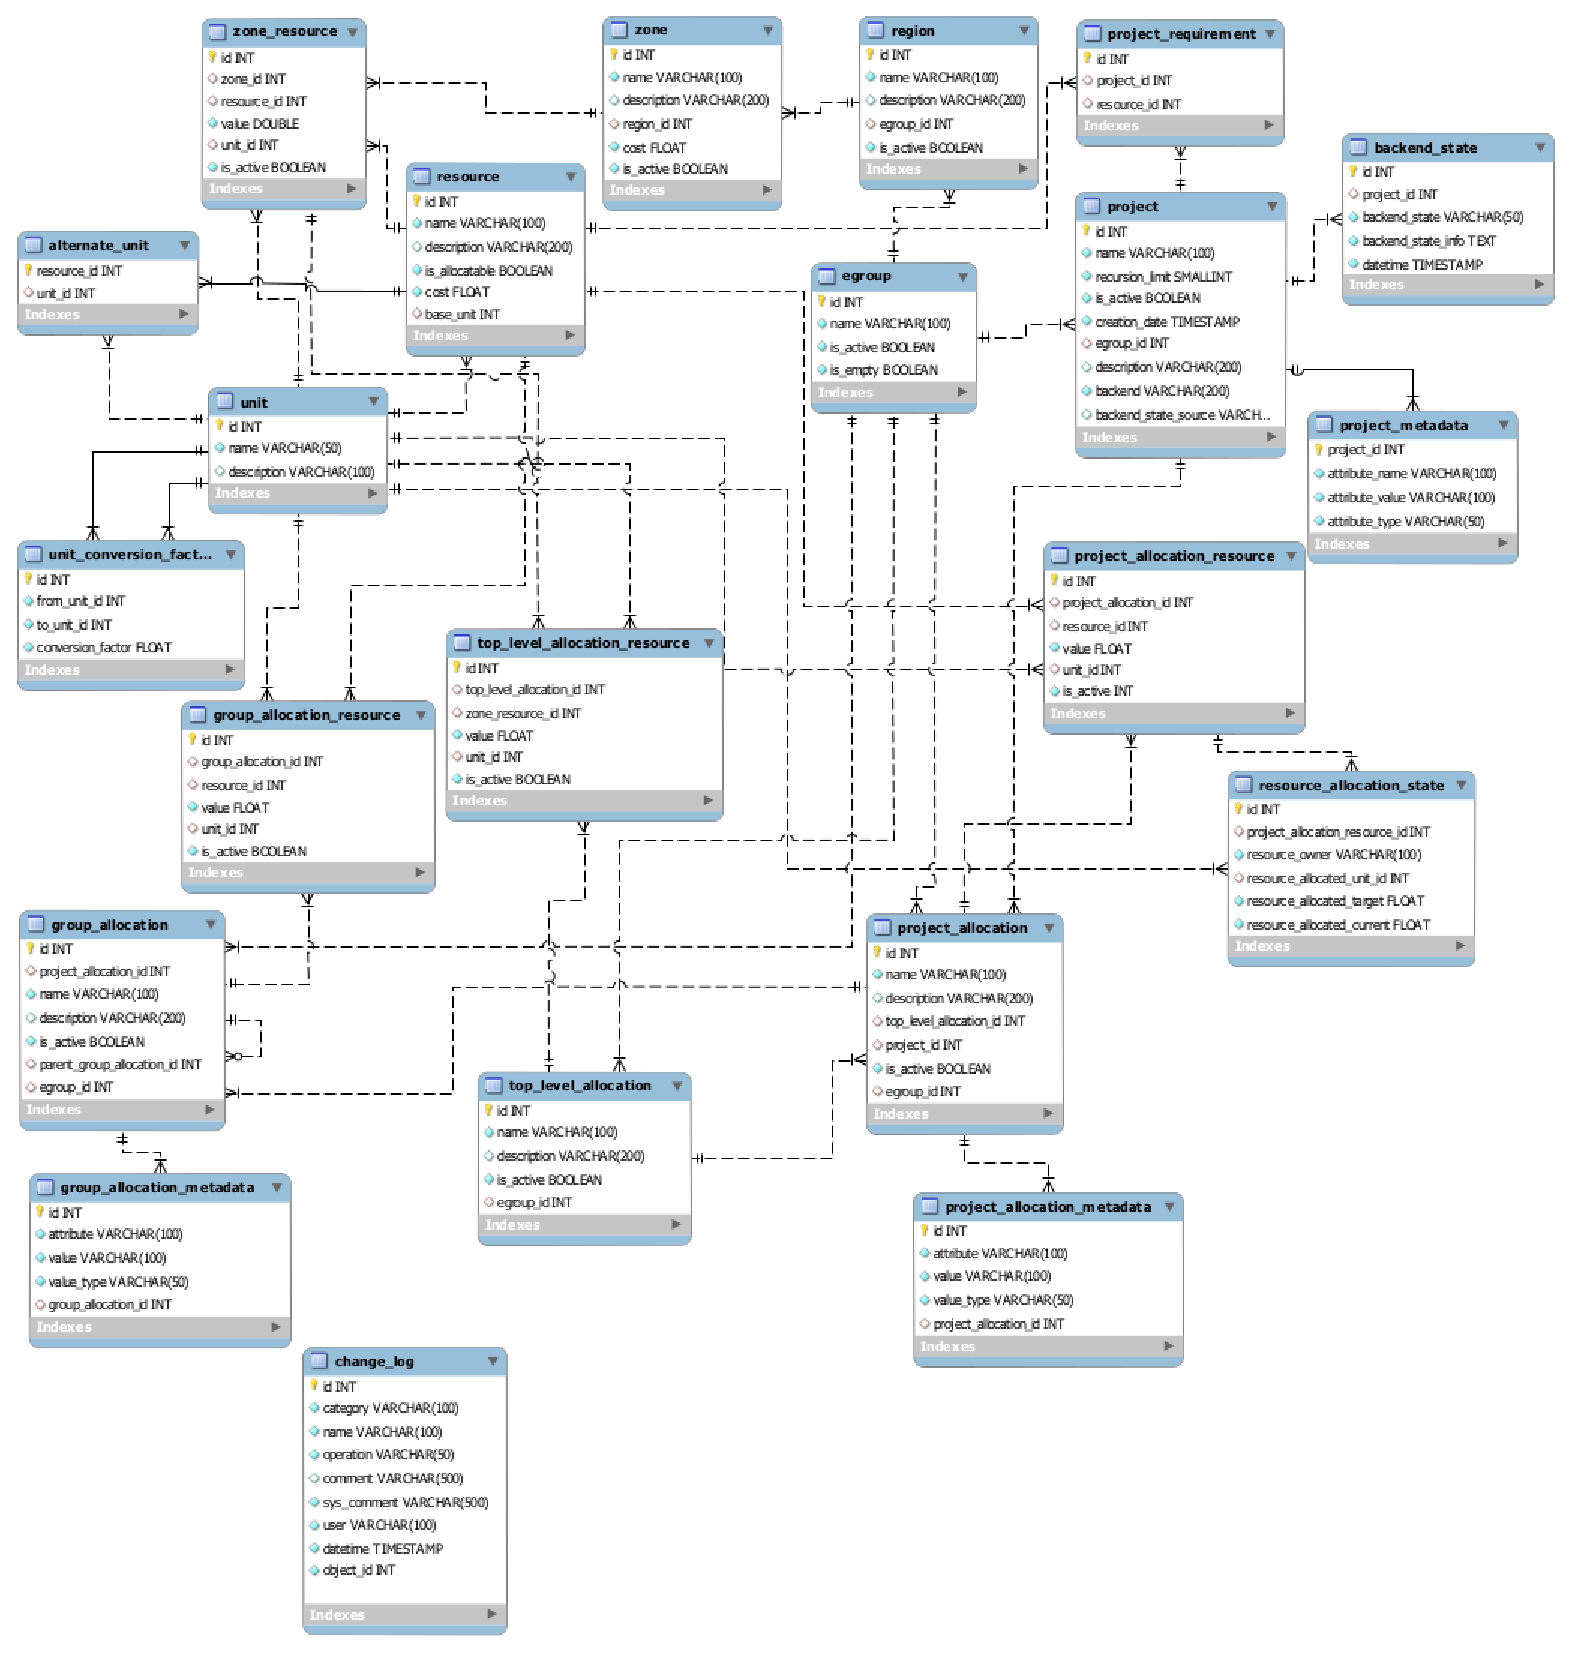
\includegraphics[width=\textwidth]{cloudman_db.eps}
\caption{\label{ddb_schema_new} Cloudman database schema, Betelgeuze release.}
\end{center}
\end{figure}

The figure ~\ref{ddb_schema_new} shows the final database schema for the FIXME:Aldebaran release of CloudMan.


The description of resources is kept in the database as well. This way, it is easy to define new valid resource attributes directly via the web interface. Updating this table is reserved to the resource manager role who owns all privileges. 

Resources and groups are matched at the top level by the resource manager in the process of filling in the allocations. Allocations are done in terms of CPU, disk and memory for each resource available. 
The resource manager approves requests for the allocations. Only approved allocations will be exported, 
and used by the back-ends.

At the lower levels, the managers do allocations out of the quota which have been allocated to them by an upper instance. 






%
% references
%
\begin{thebibliography}{99}
%
% references
%
\bibitem{ORM}
http://en.wikipedia.org/wiki/Object-relational\_mapping
\bibitem{Django}
https://www.djangoproject.com
\bibitem{CloudManProject}
CloudMan: project description, CERN IT-DEP/PES-PS, July 2011
\bibitem{CernSSO}
https://espace.cern.ch/authentication/CERN\%20Authentication\%20Help/Integrate\%20CERN\%20SSO\%20in\%20Apache.aspx
\bibitem{CernEgroups}
https://espace.cern.ch/e-groups-help/default.aspx
\bibitem{ONE}
See: http://opennebula.org
\bibitem{OPENSTACK}
See: http://opensstack.org
%\bibitem{LSF}
%Release Notes for Platform LSF Version 7.0, Nov. 2006,  PLATFORM corporation.
\bibitem{XEN}
http://www.xen.org
\bibitem{KVM}
http://www.linux-kvm.org
\bibitem{arne}
priv. comm. Arne Wiebalck, CERN-IT
\bibitem{luca}
priv. comm. Luca Mascetti, CERN-IT

\end{thebibliography}
\end{document}


